\documentclass[
11pt, % The default document font size, options: 10pt, 11pt, 12pt
%codirector, % Uncomment to add a codirector to the title page
]{charter} 




% El títulos de la memoria, se usa en la carátula y se puede usar el cualquier lugar del documento con el comando \ttitle
\titulo{Sistema de monitoreo para equipos de captura de CO$_2$} 

% Nombre del posgrado, se usa en la carátula y se puede usar el cualquier lugar del documento con el comando \degreename
%\posgrado{Carrera de Especialización en Sistemas Embebidos} 
\posgrado{Carrera de Especialización en Internet de las Cosas} 
%\posgrado{Carrera de Especialización en Intelegencia Artificial}
%\posgrado{Maestría en Sistemas Embebidos} 
%\posgrado{Maestría en Internet de las cosas}

% Tu nombre, se puede usar el cualquier lugar del documento con el comando \authorname
\autor{Ing. Alena Grebneva} 

% El nombre del director y co-director, se puede usar el cualquier lugar del documento con el comando \supname y \cosupname y \pertesupname y \pertecosupname
\director{Mg. Ing. Milton Eduardo Sosa}
\pertenenciaDirector{FIUBA} 
% FIXME:NO IMPLEMENTADO EL CODIRECTOR ni su pertenencia
\codirector{John Doe} % para que aparezca en la portada se debe descomentar la opción codirector en el documentclass
\pertenenciaCoDirector{FIUBA}

% Nombre del cliente, quien va a aprobar los resultados del proyecto, se puede usar con el comando \clientename y \empclientename
\cliente{Mg. Ing. Eddie Jose Sierra Higuerey}
\empresaCliente{Green Backbone}

% Nombre y pertenencia de los jurados, se pueden usar el cualquier lugar del documento con el comando \jurunoname, \jurdosname y \jurtresname y \perteunoname, \pertedosname y \pertetresname.
\juradoUno{Nombre y Apellido (1)}
\pertenenciaJurUno{pertenencia (1)} 
\juradoDos{Nombre y Apellido (2)}
\pertenenciaJurDos{pertenencia (2)}
\juradoTres{Nombre y Apellido (3)}
\pertenenciaJurTres{pertenencia (3)}
 
\fechaINICIO{25 de abril de 2023}		%Fecha de inicio de la cursada de GdP \fechaInicioName
\fechaFINALPlan{13 de junio de 2023} 	%Fecha de final de cursada de GdP
\fechaFINALTrabajo{Marzo de 2024}	%Fecha de defensa pública del trabajo final


\begin{document}

\maketitle
\thispagestyle{empty}
\pagebreak


\thispagestyle{empty}
{\setlength{\parskip}{0pt}
\tableofcontents{}
}
\pagebreak


\section*{Registros de cambios}
\label{sec:registro}


\begin{table}[ht]
\label{tab:registro}
\centering
\begin{tabularx}{\linewidth}{@{}|c|X|c|@{}}
\hline
\rowcolor[HTML]{C0C0C0} 
Revisión & \multicolumn{1}{c|}{\cellcolor[HTML]{C0C0C0}Detalles de los cambios realizados} & Fecha      \\ \hline
0      & Creación del documento y asignación del director		&\fechaInicioName \\ \hline
1      & Se completa hasta el punto 5 inclusive             	& 8 de mayo de 2023 \\ \hline
2      & Se completa hasta el punto 9 inclusive				& 16 de mayo de 2023 \\ \hline
%		  Se puede agregar algo más \newline
%		  En distintas líneas \newline
%		  Así                                                    & dd/mm/aaaa \\ \hline
%3      & Se completa hasta el punto 11 inclusive                & dd/mm/aaaa \\ \hline
%4      & Se completa el plan	                                 & dd/mm/aaaa \\ \hline
\end{tabularx}
\end{table}

\pagebreak



\section*{Acta de constitución del proyecto}
\label{sec:acta}

\begin{flushright}
Buenos Aires, \fechaInicioName
\end{flushright}

\vspace{1cm}

Por medio de la presente se acuerda con la \authorname\hspace{1px} que su Trabajo Final de la \degreename\hspace{1px} se titulará ``\ttitle'' y consistirá en el desarrollo de un prototipo para un sistema capaz de monitorear a distancia los equipos de captura de CO$_2$ pertenecientes al proyecto \textit{Green Backbone}, y tendrá un presupuesto preliminar estimado de 600 h de trabajo y \textcolor{red}{\$XXX}, con fecha de inicio el \fechaInicioName\hspace{1px} y fecha de presentación pública en \fechaFinalName.

Se adjunta a esta acta la planificación inicial.

\vfill

% Esta parte se construye sola con la información que hayan cargado en el preámbulo del documento y no debe modificarla
\begin{table}[ht]
\centering
\begin{tabular}{ccc}
\begin{tabular}[c]{@{}c@{}}Dr. Ing. Ariel Lutenberg \\ Director posgrado FIUBA\end{tabular} & \hspace{2cm} & \begin{tabular}[c]{@{}c@{}}\clientename \\ Fundador de \textit{\empclientename} \end{tabular} \vspace{2.5cm} \\ 
\multicolumn{3}{c}{\begin{tabular}[c]{@{}c@{}} \supname \\ Director del Trabajo Final\end{tabular}} \vspace{2.5cm} \\
%\begin{tabular}[c]{@{}c@{}}\jurunoname \\ Jurado del Trabajo Final\end{tabular}     &  & \begin{tabular}[c]{@{}c@{}}\jurdosname\\ Jurado del Trabajo Final\end{tabular}  \vspace{2.5cm}  \\
%\multicolumn{3}{c}{\begin{tabular}[c]{@{}c@{}} \jurtresname\\ Jurado del Trabajo Final\end{tabular}} \vspace{.5cm}                                                                     
\end{tabular}
\end{table}




\section{1. Descripción técnica-conceptual del proyecto a realizar}
\label{sec:descripcion}
El presente proyecto forma parte de la iniciativa de sostenibilidad \textit{Green Backbone} (en adelante GB). El objetivo de esta iniciativa es hacer frente a los efectos de la emisión de gases de efecto invernadero (GEI) y descarbonizar el aire del ambiente. 

La emisión de GEI que se produce en actividades humanas, tales como la quema de hidrocarburos y la industrialización, se asocia con el cambio climático. Estas emisiones tienen efectos perjudiciales en los sistemas naturales y en los seres humanos a nivel mundial. 

Algunos de los efectos del cambio climático son: el aumento del nivel del mar, el derretimiento de glaciares y la alteración de los patrones climáticos. Estos cambios, a su vez, pueden tener un impacto negativo sobre la seguridad alimentaria, la disponibilidad de agua y la salud de las personas. 

Para hacer frente a esta problemática algunos actores globales (países, compañías e instituciones) se comprometieron a implementar una serie de estrategias que, en primer lugar, permitan reducir gradualmente la emisión de los GEI hacia el año 2030 y luego alcanzar lo que se conoce como \textit{net zero} o emisión cero para el año 2050. 

El concepto de \textit{net zero} o neutralidad de carbono implica lograr un equilibrio entre las emisiones de GEI producidas y las emisiones que se eliminan o se compensan. Por ello, en los últimos años, han surgido iniciativas para el desarrollo de soluciones tecnológicas que permitan remover grandes cantidades de dióxido de carbono (entre 100 y 1.000 Gt de CO$_2$) presente en la atmósfera y alcanzar el \textit{net zero} más rápidamente.

El proyecto GB es liderado el Mg. Ing. Eddie Jose Sierra Higuerey y surgió en Bogotá (Colombia), en el año 2021, como uno de los participantes de la competencia global \textit{XPRIZE Carbon Removal}, donde se ofrecía un premio económico a quienes desarrollen y demuestren la eficiencia de soluciones tecnológicas para secuestrar y retener el dióxido de carbono (CO$_2$) de la atmósfera y los océanos.

Durante la competencia, los miembros del equipo de GB desarrollaron un proceso químico innovador para capturar CO$_2$ del aire y demostraron su funcionamiento en un prototipo de pequeña escala. 

En el proceso químico desarrollado, el aire del ambiente se inyecta con un compresor en un reactor que contiene desechos orgánicos y luego se lo hace circular por un tren de fotobiorreactores. El CO$_2$ queda retenido en ambas etapas del proceso y se puede comercializar como materia prima.

Para capturar grandes volúmenes de CO$_2$ mediante la implementación a gran escala del proceso desarrollado, el equipo de GB de Bogotá comenzó a construir en el año 2022 un prototipo comercial al que se denominó “GB005 Unidad Ángel”. 

Se estima que la unidad GB005 podrá capturar 3,3 toneladas de CO$_2$ al año. También permitirá validar las tecnologías, mejorar el diseño y atraer inversionistas al proyecto.

Para para esta unidad se solicitó a la autora del proyecto desarrollar un dispositivo que registre los niveles de concentración de CO$_2$ en la entrada y la salida de aire del equipo y los muestre en un display LCD, para evaluar el rendimiento del proceso de captura. 

En la figura \ref{fig:diagNodo} se muestra el diagrama en bloques del dispositivo, denominado nodo de medición, al que se adicionaron sensores de temperatura y pH para monitorear la salud de los biorreactores. También se propuso emplear un sensor de luz y relés para controlar el encendido y apagado de la unidad. 

\begin{figure}[htpb]
\centering 
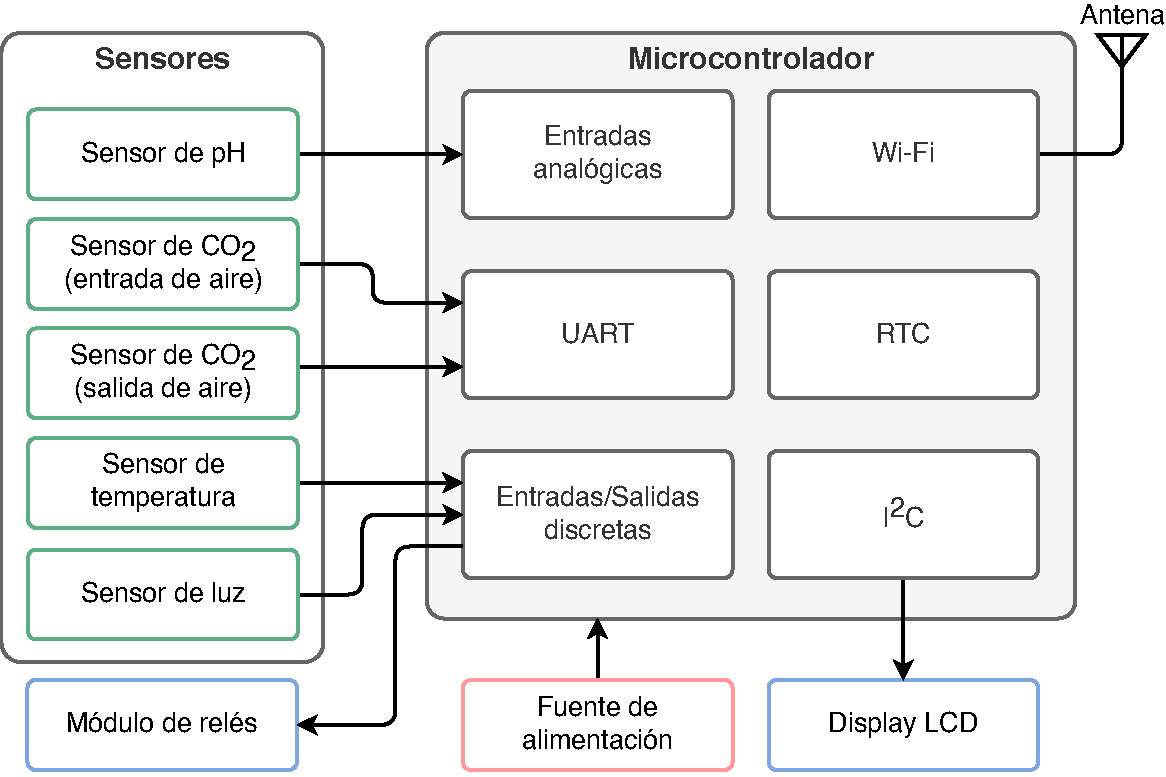
\includegraphics[width=.65\textwidth]{./Figuras/dgNodo.pdf}
\caption{Diagrama en bloques del nodo de medición.}
\label{fig:diagNodo}
\end{figure}

En una instancia de trabajo anterior al curso del posgrado se definió qué microcontrolador y sensores se van a utilizar y se propuso la conexión de todos los elementos. Asimismo, se desarrolló un firmware básico para poder monitorear los niveles de CO$_2$ y mostrar las mediciones en un display. En el presente proyecto se tomará esta base de diseño para mejorar el firmware propuesto.

A futuro, cuando se logre un diseño eficiente y se obtenga financiación, GB proyecta la construcción en serie de nuevas unidades en diferentes tamaños y capacidades de captura. Estas unidades se van a comercializar en Colombia y en el resto del mundo. Por ello, además del nodo de monitoreo para cada unidad, se necesita una plataforma capaz de recolectar y almacenar datos operativos de todas las unidades instaladas, sin importar donde se localicen físicamente.

Como la primera unidad de GB aún se encuentra en etapa de desarrollo, la propuesta del presente proyecto es un prototipo para evaluar su desempeño, agregar funciones de comunicación inalámbrica al nodo para que envíe las mediciones de los sensores hacia un broker MQTT (\textit{Message Queues Telemetry Transport}) y desarrollar la infraestructura del sistema de monitoreo.

En la figura \ref{fig:diagBloques} se muestra una arquitectura tentativa del sistema, que se compone de tres elementos principales: el nodo de medición, un broker MQTT y un entorno de desarrollo para la aplicación de monitoreo.

\begin{figure}[htpb]
\centering 
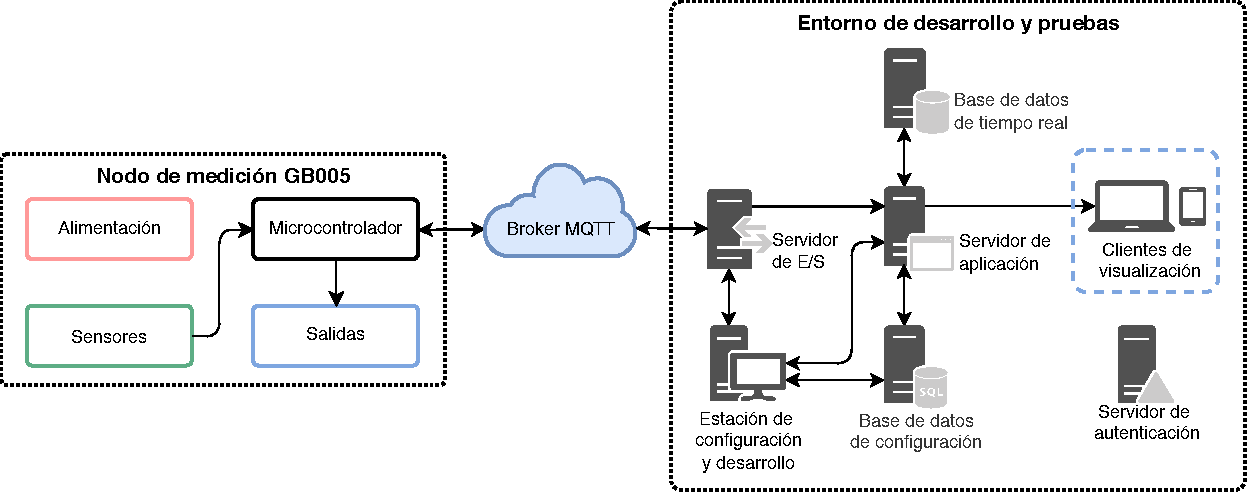
\includegraphics[width=1\textwidth]{./Figuras/diagBloques.pdf}
\caption{Arquitectura del sistema.}
\label{fig:diagBloques}
\end{figure}

El nodo de medición recolecta las emdiciones de los sensores y los envía al broker MQTT, que actúa como un intermediario entre el nodo de medición y la aplicación.

La aplicación lee los datos del broker MQTT a través del servidor de entradas y salidas. Utilizando esta información, permite visualizar el funcionamiento general de la unidad en tiempo real a través del servidor de aplicación.

Además de la visualización en tiempo real, la aplicación también almacena la información operativa en una base de datos de tiempo real. Esto permite acceder a los datos históricos y realizar análisis posteriores sobre el funcionamiento de la unidad.

Actualmente existen diferentes soluciones de mercado para implementar aplicaciones IoT. En el presente proyecto, para desarrollar el sistema de monitoreo, se empleará el software \textit{AVEVA System Platform} (ASP) ya que es una solución ampliamente utilizada en la industria con continuo desarrollo y soporte.

El ASP soporta arquitecturas de IoT mediante el uso del protocolo MQTT, posee un entorno gráfico que permite implementar aplicaciones de visualización y una base de datos histórica para almacenar las mediciones de los sensores. 

Además, se tiene acceso a una licencia de desarrollo del ASP sin cargo, ya que la autora del presente proyecto es empleada de AVEVA, la empresa que comercializa la solución. Esto permite reducir costos y tiempos de desarrollo del proyecto.

\section{2. Identificación y análisis de los interesados}
\label{sec:interesados}

\begin{table}[ht]
%\caption{Identificación de los interesados}
%\label{tab:interesados}
\begin{tabularx}{\linewidth}{|l|>{\raggedright\arraybackslash}X|>{\raggedright\arraybackslash}X|l|}
\hline
\rowcolor[HTML]{C0C0C0} 
Rol           & Nombre y Apellido & Organización 		& Puesto 	\\ \hline
%Auspiciante  & -                 & 			 		& -      	\\ \hline
Cliente       & \clientename      &Green Backbone y AVEVA	&  Fundador de GB \\ \hline
%Impulsor     &                   &              		&        	\\ \hline
Responsable   & \authorname       & FIUBA   			& Alumna 	\\ \hline
Colaboradores & -                 & -            		& Empleados de GB/AVEVA \\ \hline
Orientador    & \supname	      	 & \pertesupname 		& Director del trabajo final \\ \hline
%Equipo       & miembro1 \newline 
%				miembro2        	 &              		&        	\\ \hline
%Opositores   &                   &              		&        	\\ \hline
Usuario final & -				 & -            		&  Equipo de GB y sus clientes\\ \hline
\end{tabularx}
\end{table}
\begin{itemize}
	\item Cliente: Eddie Sierra, creó GB como emprendimiento personal y es el principal interesado en el desarrollo de la aplicación de monitoreo para mostrar el valor del proyecto. Trabaja en AVEVA y está impulsando la visibilidad del proyecto GB dentro de esta organización y empresas asociadas para conseguir financiamiento e interesados. Actualmente se ocupa de todas las cuestiones constructivas de la unidad Ángel, con lo cual no dispone de tiempo para hacer un seguimiento detallado del desarrollo. Su prioridad es que el desarrollo tenga el menor costo posible y esté en funcionamiento cuanto antes. Vive en Colombia y se debe considerar la diferencia horaria para programar reuniones con él.
	\item Orientador: Milton Sosa, ayudará con la definición de los requerimientos y alcance del proyecto. Se encuentra viviendo en Europa y se debe considerar la diferencia horaria para programar reuniones con él.
	\item Usuario final: los miembros del equipo de GB y sus clientes utilizarán la plataforma desde diferentes partes del mundo para visualizar el estado de funcionamiento y rendimiento de las unidades.
\end{itemize}


\section{3. Propósito del proyecto}
\label{sec:proposito}

Desarrollar e implementar el prototipo para una plataforma de monitoreo que permita visualizar en tiempo real y almacenar el historial de los datos operacionales de la unidad GB005 y las unidades futuras del proyecto \textit{Green Backbone}. 

El objetivo este prototipo será monitorear el estado de funcionamiento de las unidades, evaluar su rendimiento y poder programar el mantenimiento o recambio de consumibles.

\section{4. Alcance del proyecto}
\label{sec:alcance}
El proyecto incluye:
\begin{itemize}
	\item Codificación del firmware del nodo para que envíe datos mediante el protocolo MQTT
	\item Despliegue y configuración del entorno de desarrollo y pruebas
		\begin{itemize}
		\item Configuración del entorno virtual
		\item Instalación y licenciamiento del software ASP
		\item Configuración de acceso y seguridad
		\end{itemize}
	\item Configuración de la colección e historización de datos
	\item Desarrollo de la aplicación de visualización en tiempo real
	\item Desarrollo de plantillas para las unidades futuras
	
\end{itemize}

El proyecto no incluye:
\begin{itemize}
	\item Desarrollo del hardware del nodo de medición
	\item Despliegue del broker MQTT
	\item Contratación de servicios en la nube para implementar la aplicación de monitoreo
	\item Adquisición de cualquier otra licencia de software que pueda ser requerida
	\item Puesta en marcha para producción
	
\end{itemize}

\section{5. Supuestos del proyecto}
\label{sec:supuestos}

Para el desarrollo del presente proyecto se supone que: 
\begin{itemize}
	\item Se contará con los recursos económicos necesarios para realizar del proyecto
	\item Se tendrá a disposición la infraestructura de hardware necesaria para implementar la aplicación de monitoreo
	\item Se dispondrá una conexión a Internet mediante Wi-Fi continuamente para las pruebas
	\item No habrá dificultades para conseguir el software necesario (licencias, bibliotecas, certificaciones, etc)
	\item Se dispondrá del conocimiento necesario para programar el microcontrolador
	\item Se dispondrá del conocimiento para desarrollar la aplicación de monitoreo
	\item Se contará con la colaboración de profesionales idóneos en temas de conectividad, programación del microcontrolador y desarrollo de aplicaciones con el ASP, para obtener un resultado de buena calidad
	\item El cliente aceptará que algunas mediciones sean simuladas por no disponer de los sensores localmente
\end{itemize}

\section{6. Requerimientos}
\label{sec:requerimientos}

\begin{enumerate}
	\item Requerimientos de \textit{firmware} del nodo de medición
		\begin{enumerate}
			\item Disponer de conexión a una red Wi-Fi en el sitio para pruebas
			\item Envío y recepción de datos mediante el protocolo MQTT, utilizando certificados SSL/TLS para la comunicación con el broker
			\item Obtención de información horaria desde un servidor NTP
			\item Lectura de las mediciones de CO$_2$ de dos sensores MH-Z19B (correspondientes a la entrada y salida de aire) empleando la UART
			\item Lectura de la medición de temperatura de un sensor DS18B20, utilizando el protocolo \textit{One Wire}
			\item Lectura de la medición del pH de un sensor con salida analógica, mediante el ADC del microcontrolador
			\item Detección de luz diurna a través de un sensor conectado a una entrada discreta
			\item Accionamiento de dos relés mediante salidas discretas, para encender y apagar los compresores
			\item Visualización de las mediciones en un display LCD conectado al puerto I$^2$C
		\end{enumerate}
	\item Requerimientos funcionales del broker MQTT
		\begin{enumerate}
			\item Proveer certificados SSL/TLS para la comunicación del microcontrolador y la aplicación de monitoreo
			\item Ser capaz de manejar múltiples conexiones simultáneas de nodos de monitoreo
			\item Ser de acceso público
		\end{enumerate}
	\item Requerimientos de la aplicación de monitoreo
		\begin{enumerate}
			\item Envío y recepción de datos mediante el protocolo MQTT, utilizando certificados SSL/TLS para la comunicación con el broker
			\item Organización de los datos recibidos en una estructura jerárquica
			\item Visualización de las mediciones en tiempo real 
			\item Registro de las mediciones obtenidas en una base de datos
			\item Autenticación de los usuarios y control de acceso a las funcionalidades
			\item Escalabilidad para agregar nuevas unidades de GB a futuro
			\item Generación de alarmas cuando se superen los umbrales definidos para las mediciones
			\item Configuración de los umbrales de alarma
			\item Exportación de los datos en diferentes formatos
			\item Manejo de errores de comunicación con el broker MQTT y con la base de datos
		\end{enumerate}	
	\item Requerimientos de la interfaz de visualización
		\begin{enumerate}
			\item Mostrar las mediciones de los sensores en tiempo real de manera gráfica
			\item Permitir la visualización de datos históricos
			\item Ser fácil de usar para cualquier usuario sin conocimientos técnicos especializados
			\item Comunicarse con la aplicación de monitoreo mediante un protocolo de comunicación seguro 
			\item Mostrar alertas y notificaciones de las alarmas generadas
			\item Ser accesible desde cualquier dispositivo con conexión a Internet y compatible con diferentes navegadores
			\item Proteger los datos mediante autenticación y autorización de usuarios
			
		\end{enumerate}	
	\item Requerimientos de \textit{testing}
		\begin{enumerate}
			\item Se deberán realizar pruebas de funcionalidad para verificar que el nodo de monitoreo, el broker MQTT, y la aplicación de monitoreo funcionen correctamente
			\item Se deberán realizar pruebas de integración para verificar que los diferentes componentes del sistema funcionen correctamente en conjunto
			\item Se deberán realizar pruebas de rendimiento para verificar que el sistema sea capaz de enviar y procesar los datos de forma eficiente
			\item Se deberán realizar pruebas de seguridad para verificar que el sistema sea seguro y no tenga vulnerabilidades que puedan ser explotadas
		\end{enumerate}	
\end{enumerate}

\section{7. Historias de usuarios (\textit{Product backlog})}
\label{sec:backlog}
\begin{enumerate}
\item Como miembro del equipo de GB, quiero registrar los niveles de concentración de CO$_2$ en la entrada y la salida de aire de la unidad, para evaluar el rendimiento del proceso de captura.
\textit{Story points}: 8 (complejidad: 3, dificultad: 2, incertidumbre: 3)

\item Como miembro del equipo de GB, quiero que la unidad tenga conexión a Internet y envíe los datos de los sensores a una plataforma de monitoreo centralizada.

\textit{Story points}: 13 (complejidad: 5, dificultad: 3, incertidumbre: 5)

\item Como miembro del equipo de GB, quiero acceder a un registro histórico de las lecturas y alarmas generadas por cada unidad, para poder analizar su comportamiento en el largo plazo. 

\textit{Story points}: 8 (complejidad: 3, dificultad: 3, incertidumbre: 1)

\item Como miembro del equipo de GB, quiero que la plataforma de monitoreo sea segura y proteja los datos recolectados por los nodos de medición, para evitar posibles ataques o filtraciones de información. 

\textit{Story points}: 13 (complejidad: 5, dificultad: 5, incertidumbre: 3)

\item Como usuario, quiero ver los datos de funcionamiento y estadísticas sobre el rendimiento de mi unidad, desde una interfaz fácil de usar. 

\textit{Story points}: 13 (complejidad: 5, dificultad: 5, incertidumbre: 2)

\item Como usuario, quiero que el sistema de monitoreo me muestre alarmas cuando se detecten niveles de concentración de CO$_2$ en la entrada o salida de aire por encima o por debajo de ciertos umbrales. 

\textit{Story points}: 8 (complejidad: 2, dificultad: 3, incertidumbre: 3)

\item Como ingeniero de mantenimiento, quiero que el dispositivo registre y muestre en tiempo real la temperatura y el pH de los biorreactores de la unidad, para monitorear su funcionamiento y programar el cambio de consumibles.

\textit{Story points}: 13 (complejidad: 5, dificultad: 5, incertidumbre: 2)

\item Como ingeniero de mantenimiento, quiero que la unidad funcione solo durante las horas del día en que hay luz solar disponible para ahorrar energía y consumibles.

\textit{Story points}: 8 (complejidad: 3, dificultad: 2, incertidumbre: 3)

\item Como ingeniero de desarrollo, quiero garantizar que la plataforma sea escalable para incorporar nuevas unidades, a medida que se expande el negocio de \textit{Green Backbone}. 

\textit{Story points}: 8 (complejidad: 3, dificultad: 2, incertidumbre: 3)

\item Como ingeniero de desarrollo, quiero poder asignar roles y permisos de usuario para garantizar que los datos sean accesibles solo para personas autorizadas. 

\textit{Story points}: 8 (complejidad: 2, dificultad: 5, incertidumbre: 1)

\item Como científico de datos quiero que la plataforma de monitoreo tenga la capacidad de generar informes para poder analizar los datos operativos de manera detallada. 

\textit{Story points}: 13 (complejidad: 5, dificultad: 3, incertidumbre: 3)
\end{enumerate}

Para determinar los \textit{story points} de una historia de usuario, se asignaron valores a cada uno de los siguientes aspectos:
\begin{itemize}
\item Complejidad del trabajo:
	\begin{itemize}
	\item Alta: 13
	\item Media: 5
	\item Baja: 1
	\end{itemize}
\item Dificultad del trabajo:
	\begin{itemize}
	\item Alta: 5
	\item Media: 3
	\item Baja: 1
	\end{itemize}
\item Incertidumbre del trabajo:
	\begin{itemize}
	\item Alta: 5
	\item Media: 3
	\item Baja: 1
	\end{itemize}
\end{itemize}

Para obtener los \textit{story points}, se sumaron los valores asignados a cada aspecto y se aproximaron al siguiente número de la serie de Fibonacci.

Por ejemplo, si la complejidad del trabajo es media (5), la dificultad es alta (5) y la incertidumbre es media (3), los \textit{story points} serían 21 (5 + 5 + 3 = 13, que se aproxima al siguiente número de Fibonacci, que es 21).

\section{8. Entregables principales del proyecto}
\label{sec:entregables}
\begin{itemize}
\item Firmware mejorado para el nodo de medición, que permitirá enviar mediciones de los sensores hacia un broker MQTT y podrá ser utilizado para futuras unidades de GB

\item Sistema de monitoreo para la unidad GB005, que permitirá visualizar en tiempo real las mediciones de CO$_2$, temperatura, pH y luz, así como el estado de encendido y apagado de la unidad

\item Plataforma para recolectar y almacenar datos operativos de todas las unidades instaladas de GB, capaz de recibir datos de los nodos de medición mediante un broker MQTT y mostrarlos en una interfaz de usuario

\item Documentación técnica del proyecto, incluyendo diagramas y esquemáticos de conexión, listados de componentes, código fuente del firmware y archivos de backup del sistema de monitoreo
\end{itemize}
\section{9. Desglose del trabajo en tareas}
\label{sec:wbs}
\begin{enumerate}
	\item Gestión de proyecto (50 horas)
	\begin{enumerate}
		\item Reuniones con el cliente y con el director del trabajo (10 h)
		\item Elaboración del plan de proyecto de Trabajo Final (20 h)
		\item Elaboración de la presentación del plan de proyecto (10 h)
		\item Revisión y correcciones de los entregables (10 h)
	\end{enumerate}
	\item Investigación preliminar y aprendizaje de tecnologías (120 h)
	\begin{enumerate}
		\item Protocolos de comunicación (40 h)
		\item Lenguajes de programación (40 h)
		\item Herramientas de desarrollo (40 h)
	\end{enumerate}
		\item Desarrollo del firmware para el microcontrolador (111 h)
	\begin{enumerate}
		\item Portar desarrollo existente en el \textit{framework} Arduino al de ESP-IDF (10 h)
		\item Programación de la conexión Wi-Fi y configuración de la red (5 h)
		\item Implementación del protocolo MQTT con certificados SSL/TLS (20 h)
		\item Integración del servidor NTP para obtener información horaria (2 h)
		\item Programación de la adquisición de mediciones (34 h)
		\begin{enumerate}[label*=\arabic*.,ref=\theenumii.\arabic*]
			\item Definición de conexiones entre el microcontrolador y los sensores (10 h)
			\item Lectura de niveles de CO$_2$ desde los sensores MH-Z19B (5 h)
			\item Lectura de la temperatura del sensor DS18B20 (5 h)
			\item Simulación de la medición del pH (5 h)
			\item Detección de luz diurna (2 h)
			\item Accionamiento de los relés (2 h)
			\item Visualización de las mediciones en el display LCD (5 h)
		\end{enumerate}
		\item Pruebas de adquisición de datos de todos los sensores disponibles (10 h)
		\item Pruebas de envío de mediciones de todos los sensores al broker MQTT (10 h)
		\item Corrección de errores (20 h)
	\end{enumerate}
	\item Desarrollo del \textit{backend} de la aplicación de monitoreo (165 h)
	\begin{enumerate}
		\item Configuración del entorno de desarrollo y pruebas (20 h)
		\item Instalación y licenciamiento del software ASP (10 h)
		\item Configuración de acceso y seguridad en el ASP (15 h)
		\item Modelado de la aplicación mediante objetos (40 h)
		\item Configuración de la adquisición de datos mediante el driver MQTT (20 h)
		\item Configuración de la historización de datos (10 h)
		\item Despliegue del \textit{runtime} de la aplicación (10 h)
		\item Pruebas de adquisición de datos (10 h)
		\item Pruebas de funcionamiento en \textit{runtime} (10 h)
		\item Corrección de errores (20 h)
	\end{enumerate}
	\item Desarrollo del \textit{frontend} de la aplicación de monitoreo (130 h)
	\begin{enumerate}
		\item Diseño del \textit{layout} de la interfaz de usuario (20 h)
		\item Implementación de la visualización de datos en tiempo real (30 h)
		\item Implementación de la visualización de datos históricos (10 h)
		\item Implementación del acceso remoto a la aplicación de visualización (20 h)
		\item Implementación de reportes (20 h)
		\item Pruebas de funcionamiento en \textit{runtime} (10 h)
		\item Corrección de errores (20 h)
	\end{enumerate}
	\item Generación de entregables y proceso de cierre (80 horas)
	\begin{enumerate}
		\item Elaboración del informe de avance (15 horas)
		\item Elaboración memoria técnica de Trabajo Final (40 h)
		\item Revisión y correcciones de la memoria (10 h)
		\item Elaboración de la presentación final (8 h)
		\item Revisión y correcciones de la presentación final (2 h)
	\end{enumerate}
\end{enumerate}

Cantidad total de horas: 656 h.

\section{10. Diagrama de Activity On Node}
\label{sec:AoN}

\begin{consigna}{red}
Armar el AoN a partir del WBS definido en la etapa anterior. 

%La figura \ref{fig:AoN} fue elaborada con el paquete latex tikz y pueden consultar la siguiente referencia \textit{online}:

%\url{https://www.overleaf.com/learn/latex/LaTeX_Graphics_using_TikZ:_A_Tutorial_for_Beginners_(Part_3)\%E2\%80\%94Creating_Flowcharts}

\end{consigna}

\begin{figure}[htpb]
\centering 
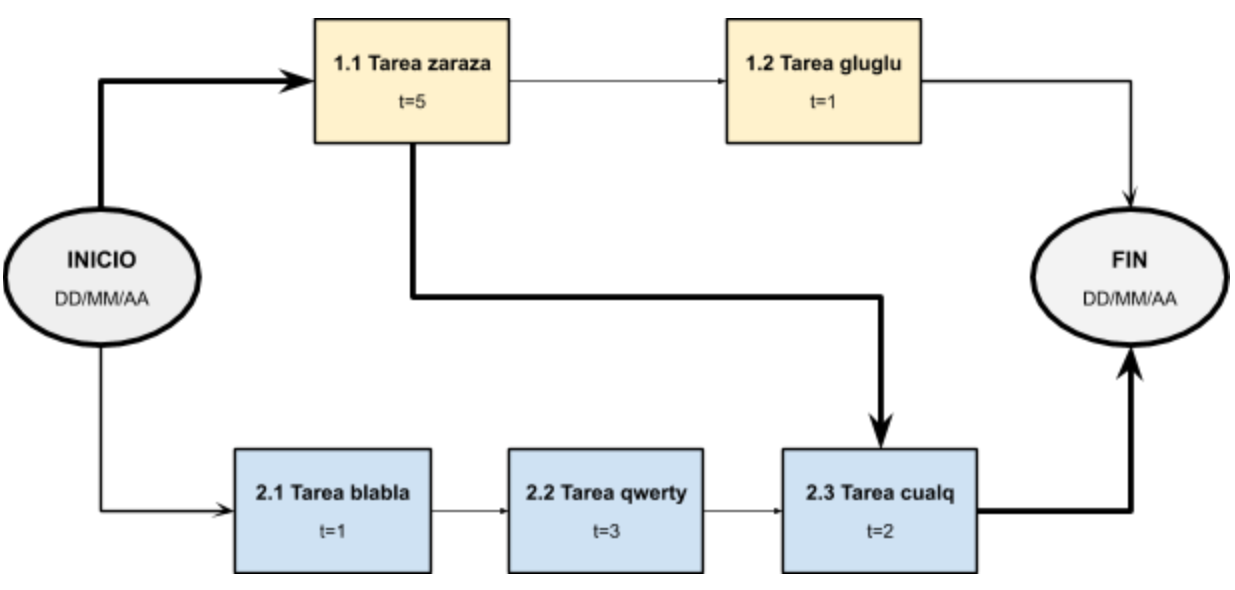
\includegraphics[width=.8\textwidth]{./Figuras/AoN.png}
\caption{Diagrama de \textit{Activity on Node}.}
\label{fig:AoN}
\end{figure}

Indicar claramente en qué unidades están expresados los tiempos.
De ser necesario indicar los caminos semicríticos y analizar sus tiempos mediante un cuadro.
Es recomendable usar colores y un cuadro indicativo describiendo qué representa cada color, como se muestra en el siguiente ejemplo:



\section{11. Diagrama de Gantt}
\label{sec:gantt}

\begin{consigna}{red}

Existen muchos programas y recursos \textit{online} para hacer diagramas de Gantt, entre los cuales destacamos:

\begin{itemize}
\item Planner
\item GanttProject
\item Trello + \textit{plugins}. En el siguiente link hay un tutorial oficial: \\ \url{https://blog.trello.com/es/diagrama-de-gantt-de-un-proyecto}
\item Creately, herramienta online colaborativa. \\\url{https://creately.com/diagram/example/ieb3p3ml/LaTeX}
\item Se puede hacer en latex con el paquete \textit{pgfgantt}\\ \url{http://ctan.dcc.uchile.cl/graphics/pgf/contrib/pgfgantt/pgfgantt.pdf}
\end{itemize}

Pegar acá una captura de pantalla del diagrama de Gantt, cuidando que la letra sea suficientemente grande como para ser legible. 
Si el diagrama queda demasiado ancho, se puede pegar primero la ``tabla'' del Gantt y luego pegar la parte del diagrama de barras del diagrama de Gantt.

Configurar el software para que en la parte de la tabla muestre los códigos del EDT (WBS).\\
Configurar el software para que al lado de cada barra muestre el nombre de cada tarea.\\
Revisar que la fecha de finalización coincida con lo indicado en el Acta Constitutiva.

En la figura \ref{fig:gantt}, se muestra un ejemplo de diagrama de Gantt realizado con el paquete de \textit{pgfgantt}. En la plantilla pueden ver el código que lo genera y usarlo de base para construir el propio.

\begin{figure}[htbp]
\begin{center}
\begin{ganttchart}{1}{12}
  \gantttitle{2020}{12} \\
  \gantttitlelist{1,...,12}{1} \\
  \ganttgroup{Group 1}{1}{7} \\
  \ganttbar{Task 1}{1}{2} \\
  \ganttlinkedbar{Task 2}{3}{7} \ganttnewline
  \ganttmilestone{Milestone o hito}{7} \ganttnewline
  \ganttbar{Final Task}{8}{12}
  \ganttlink{elem2}{elem3}
  \ganttlink{elem3}{elem4}
\end{ganttchart}
\end{center}
\caption{Diagrama de Gantt de ejemplo}
\label{fig:gantt}
\end{figure}


\begin{landscape}
\begin{figure}[htpb]
\centering 
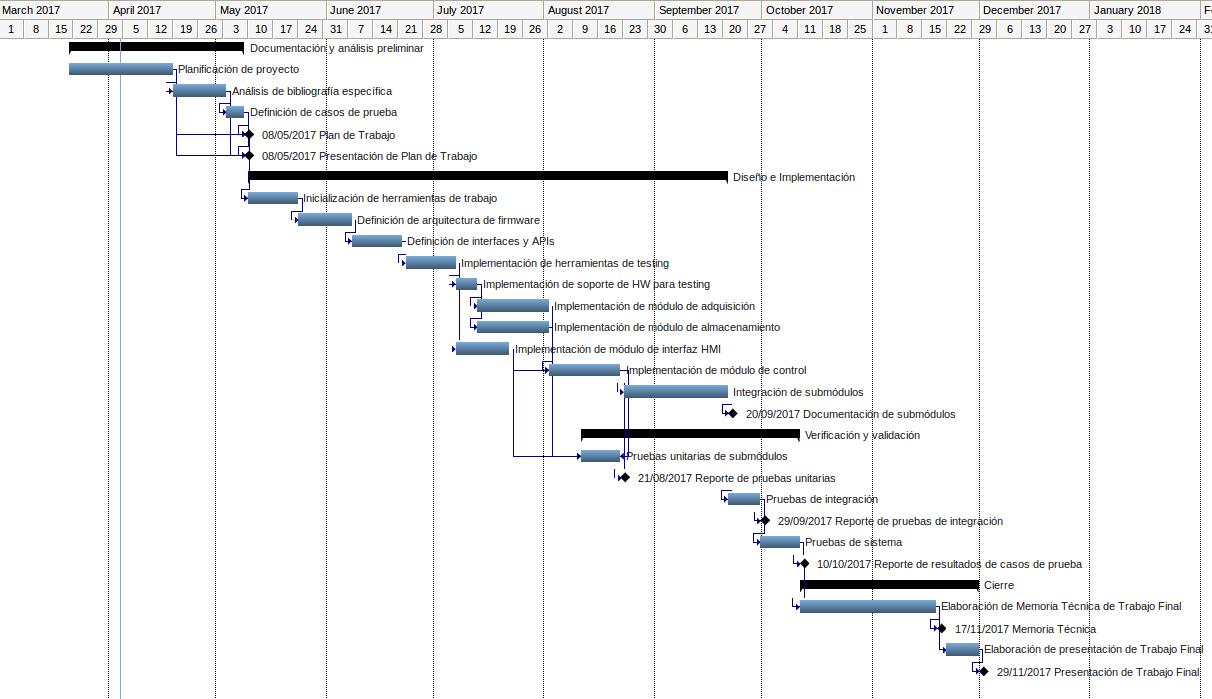
\includegraphics[height=.85\textheight]{./Figuras/Gantt-2.png}
\caption{Ejemplo de diagrama de Gantt rotado}
\label{fig:diagGantt}
\end{figure}

\end{landscape}

\end{consigna}


\section{12. Presupuesto detallado del proyecto}
\label{sec:presupuesto}

\begin{consigna}{red}
Si el proyecto es complejo entonces separarlo en partes:
\begin{itemize}
	\item Un total global, indicando el subtotal acumulado por cada una de las áreas.
	\item El desglose detallado del subtotal de cada una de las áreas.
\end{itemize}

IMPORTANTE: No olvidarse de considerar los COSTOS INDIRECTOS.

\end{consigna}

\begin{table}[htpb]
\centering
\begin{tabularx}{\linewidth}{@{}|X|c|r|r|@{}}
\hline
\rowcolor[HTML]{C0C0C0} 
\multicolumn{4}{|c|}{\cellcolor[HTML]{C0C0C0}COSTOS DIRECTOS} \\ \hline
\rowcolor[HTML]{C0C0C0} 
Descripción &
  \multicolumn{1}{c|}{\cellcolor[HTML]{C0C0C0}Cantidad} &
  \multicolumn{1}{c|}{\cellcolor[HTML]{C0C0C0}Valor unitario} &
  \multicolumn{1}{c|}{\cellcolor[HTML]{C0C0C0}Valor total} \\ \hline
 &
  \multicolumn{1}{c|}{} &
  \multicolumn{1}{c|}{} &
  \multicolumn{1}{c|}{} \\ \hline
 &
  \multicolumn{1}{c|}{} &
  \multicolumn{1}{c|}{} &
  \multicolumn{1}{c|}{} \\ \hline
\multicolumn{1}{|l|}{} &
   &
   &
   \\ \hline
\multicolumn{1}{|l|}{} &
   &
   &
   \\ \hline
\multicolumn{3}{|c|}{SUBTOTAL} &
  \multicolumn{1}{c|}{} \\ \hline
\rowcolor[HTML]{C0C0C0} 
\multicolumn{4}{|c|}{\cellcolor[HTML]{C0C0C0}COSTOS INDIRECTOS} \\ \hline
\rowcolor[HTML]{C0C0C0} 
Descripción &
  \multicolumn{1}{c|}{\cellcolor[HTML]{C0C0C0}Cantidad} &
  \multicolumn{1}{c|}{\cellcolor[HTML]{C0C0C0}Valor unitario} &
  \multicolumn{1}{c|}{\cellcolor[HTML]{C0C0C0}Valor total} \\ \hline
\multicolumn{1}{|l|}{} &
   &
   &
   \\ \hline
\multicolumn{1}{|l|}{} &
   &
   &
   \\ \hline
\multicolumn{1}{|l|}{} &
   &
   &
   \\ \hline
\multicolumn{3}{|c|}{SUBTOTAL} &
  \multicolumn{1}{c|}{} \\ \hline
\rowcolor[HTML]{C0C0C0}
\multicolumn{3}{|c|}{TOTAL} &
   \\ \hline
\end{tabularx}%
\end{table}


\section{13. Gestión de riesgos}
\label{sec:riesgos}

\begin{consigna}{red}
a) Identificación de los riesgos (al menos cinco) y estimación de sus consecuencias:
 
Riesgo 1: detallar el riesgo (riesgo es algo que si ocurre altera los planes previstos de forma negativa)
\begin{itemize}
	\item Severidad (S): mientras más severo, más alto es el número (usar números del 1 al 10).\\
	Justificar el motivo por el cual se asigna determinado número de severidad (S).
	\item Probabilidad de ocurrencia (O): mientras más probable, más alto es el número (usar del 1 al 10).\\
	Justificar el motivo por el cual se asigna determinado número de (O). 
\end{itemize}   

Riesgo 2:
\begin{itemize}
	\item Severidad (S): 
	\item Ocurrencia (O):
\end{itemize}

Riesgo 3:
\begin{itemize}
	\item Severidad (S): 
	\item Ocurrencia (O):
\end{itemize}


b) Tabla de gestión de riesgos:      (El RPN se calcula como RPN=SxO)

\begin{table}[htpb]
\centering
\begin{tabularx}{\linewidth}{@{}|X|c|c|c|c|c|c|@{}}
\hline
\rowcolor[HTML]{C0C0C0} 
Riesgo & S & O & RPN & S* & O* & RPN* \\ \hline
       &   &   &     &    &    &      \\ \hline
       &   &   &     &    &    &      \\ \hline
       &   &   &     &    &    &      \\ \hline
       &   &   &     &    &    &      \\ \hline
       &   &   &     &    &    &      \\ \hline
\end{tabularx}%
\end{table}

Criterio adoptado: 
Se tomarán medidas de mitigación en los riesgos cuyos números de RPN sean mayores a...

Nota: los valores marcados con (*) en la tabla corresponden luego de haber aplicado la mitigación.

c) Plan de mitigación de los riesgos que originalmente excedían el RPN máximo establecido:
 
Riesgo 1: plan de mitigación (si por el RPN fuera necesario elaborar un plan de mitigación).
  Nueva asignación de S y O, con su respectiva justificación:
  - Severidad (S): mientras más severo, más alto es el número (usar números del 1 al 10).
          Justificar el motivo por el cual se asigna determinado número de severidad (S).
  - Probabilidad de ocurrencia (O): mientras más probable, más alto es el número (usar del 1 al 10).
          Justificar el motivo por el cual se asigna determinado número de (O).

Riesgo 2: plan de mitigación (si por el RPN fuera necesario elaborar un plan de mitigación).
 
Riesgo 3: plan de mitigación (si por el RPN fuera necesario elaborar un plan de mitigación).

\end{consigna}


\section{14. Gestión de la calidad}
\label{sec:calidad}

\begin{consigna}{red}
Elija al menos diez requerientos que a su criterio sean los más importantes/críticos/que aportan más valor y para cada uno de ellos indique las acciones de verificación y validación que permitan asegurar su cumplimiento.

\begin{itemize} 
\item Req \#1: copiar acá el requerimiento.

\begin{itemize}
	\item Verificación para confirmar si se cumplió con lo requerido antes de mostrar el sistema al cliente. Detallar 
	\item Validación con el cliente para confirmar que está de acuerdo en que se cumplió con lo requerido. Detallar  
\end{itemize}

\end{itemize}

Tener en cuenta que en este contexto se pueden mencionar simulaciones, cálculos, revisión de hojas de datos, consulta con expertos, mediciones, etc.  Las acciones de verificación suelen considerar al entregable como ``caja blanca'', es decir se conoce en profundidad su funcionamiento interno.  En cambio, las acciones de validación suelen considerar al entregable como ``caja negra'', es decir, que no se conocen los detalles de su funcionamiento interno.

\end{consigna}

\section{15. Procesos de cierre}    
\label{sec:cierre}

\begin{consigna}{red}
Establecer las pautas de trabajo para realizar una reunión final de evaluación del proyecto, tal que contemple las siguientes actividades:

\begin{itemize}
	\item Pautas de trabajo que se seguirán para analizar si se respetó el Plan de Proyecto original:
	 - Indicar quién se ocupará de hacer esto y cuál será el procedimiento a aplicar. 
	\item Identificación de las técnicas y procedimientos útiles e inútiles que se emplearon, y los problemas que surgieron y cómo se solucionaron:
	 - Indicar quién se ocupará de hacer esto y cuál será el procedimiento para dejar registro.
	\item Indicar quién organizará el acto de agradecimiento a todos los interesados, y en especial al equipo de trabajo y colaboradores:
	  - Indicar esto y quién financiará los gastos correspondientes.
\end{itemize}

\end{consigna}


\end{document}
